\documentclass{article}
\usepackage[utf8]{inputenc}
\usepackage{booktabs}
\usepackage{geometry}
\usepackage{natbib}
\usepackage{graphicx}
\usepackage{float}
\usepackage{multirow}
\usepackage{subfigure}
\usepackage{listings}
\geometry{a4paper,left=2cm,right=2cm,top=2cm,bottom=2cm}
\title{Programming Assignment 1}
\author{Dong Jing 515370910182,}
\date{September 2017}



\begin{document}

\begin{titlepage}

\begin{center}


% Upper part of the page
\textsc{\LARGE }
 \\[3cm]

\textsc{\LARGE VE281}\\[5cm]

\textsc{\Large P1 REPORT}\\[5cm]


% Title
\textsc{by}\\[1cm]
\textsc{\Large Dong Jing 515370910182}\\[0.5cm]



% Bottom of the page
{\large \today}

\end{center}

\end{titlepage}
\section{Object}
I. Study the performances of six sorting algorithms with different input size;\\
II. Compare the results and have a better understanding about sorting algorithms;\\
\section{Design}
Note: all program are executed on Ubuntu (64-bit) with memory equal to 2048 MB on Oracle VM VirtualBox 5.1.22 r115126.\\
\\
Use mrand48() to generate random arrays. And then use six sorting algorithms to sort same array and record time. Try six input sizes, 10, 50, 100, 500, 1000, 5000, 10000, 50000 and 100000. For every input size, to avoid the influence of runtime from the detailed input array, I use 50 different arrays of same input size to compute the mean runtime, which can make the result more accurate.\\
\section{Result}
Table 1 shows are data we recorded. The unit of all data is CLOCK\_PER\_SEC.\\
\begin{table}[!hbp]
\centering
\begin{tabular}{|c||c|c|c|c|c|c|}
\hline
Input size & Bubble sort & Insertion sort & Selection sort & Merge sort & Quick sort  & Quick sort \\
 & & & & & with extra array & with in-place partitioning\\
\hline
10     & 4 & 0 & 0 & 1 & 10 & 10\\
50     & 10 & 4 & 6 & 7 & 48 & 45 \\
100    & 31 & 9 & 19 & 12 & 93 & 95 \\
500    & 731 & 223 & 404 & 82 & 536 & 506 \\
1000   & 3685 & 1019 & 1866 & 193 & 1174 & 1145 \\
5000   & 112788 & 37153 & 50975 & 1245 & 8150 & 7424 \\
10000  & 835026 & 112935 & 325789 & 8967 & 22590 & 16126 \\
50000  & 17817515 & 3299634 & 5269035 & 42050 & 222990 & 187324 \\
100000 & 61788652 & 15795805 & 29900281 & 41445 & 243163 & 256087 \\
\hline
\end{tabular}
\caption{Mean runtime of different input size for six sorting algorithm.}
\end{table}
Figure 1, Figure 2 and Figure 3 show the comparisons between different sorting algorithms. They have different scale of x-axis and y-axis so that we can see the difference more directly.\\
\begin{figure}[H]
\centering
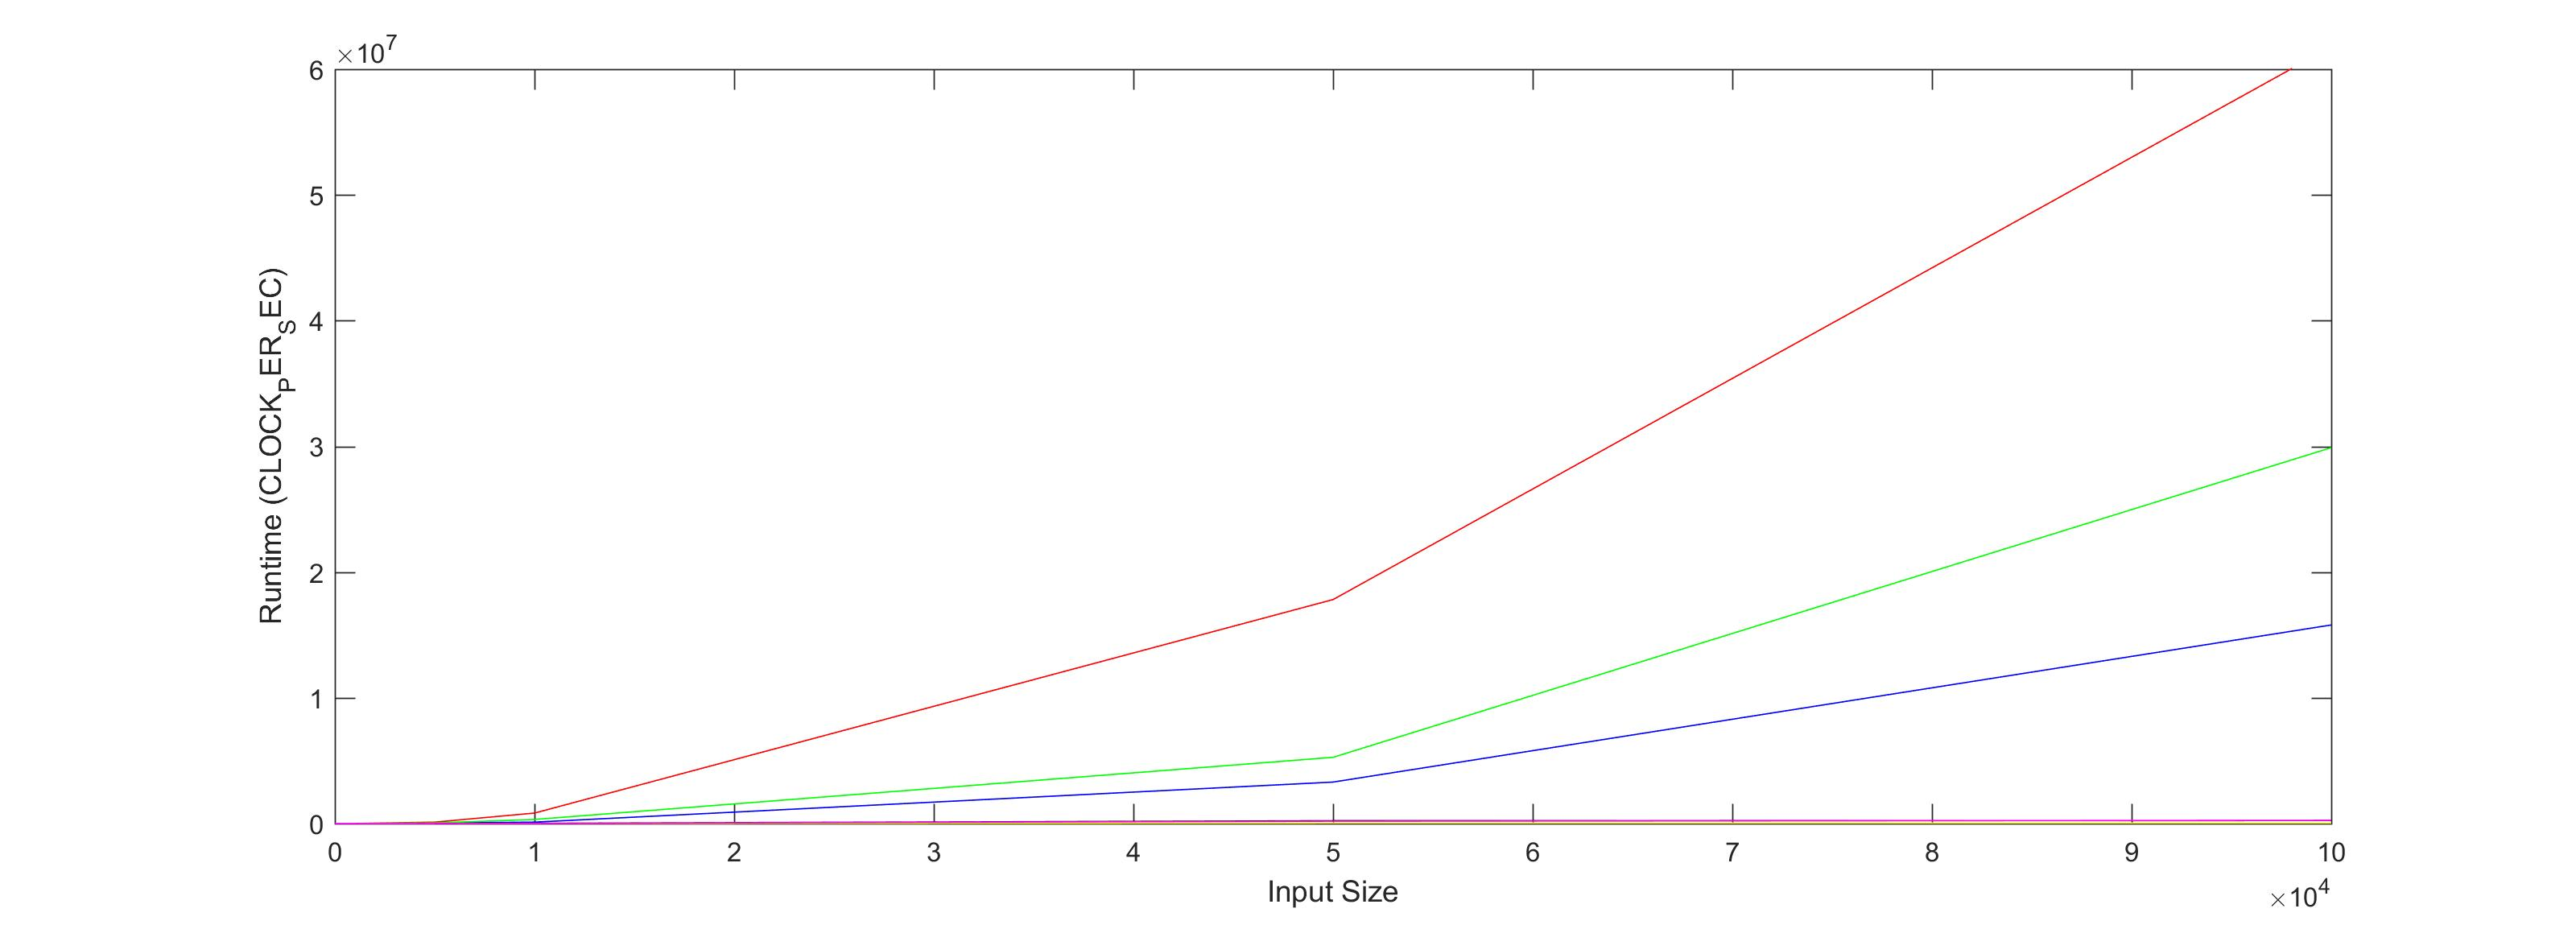
\includegraphics[width=\textwidth]{1.jpg}
\caption{Runtime of each algorithm versus the array size.}
\end{figure}
\begin{figure}[H]
\centering
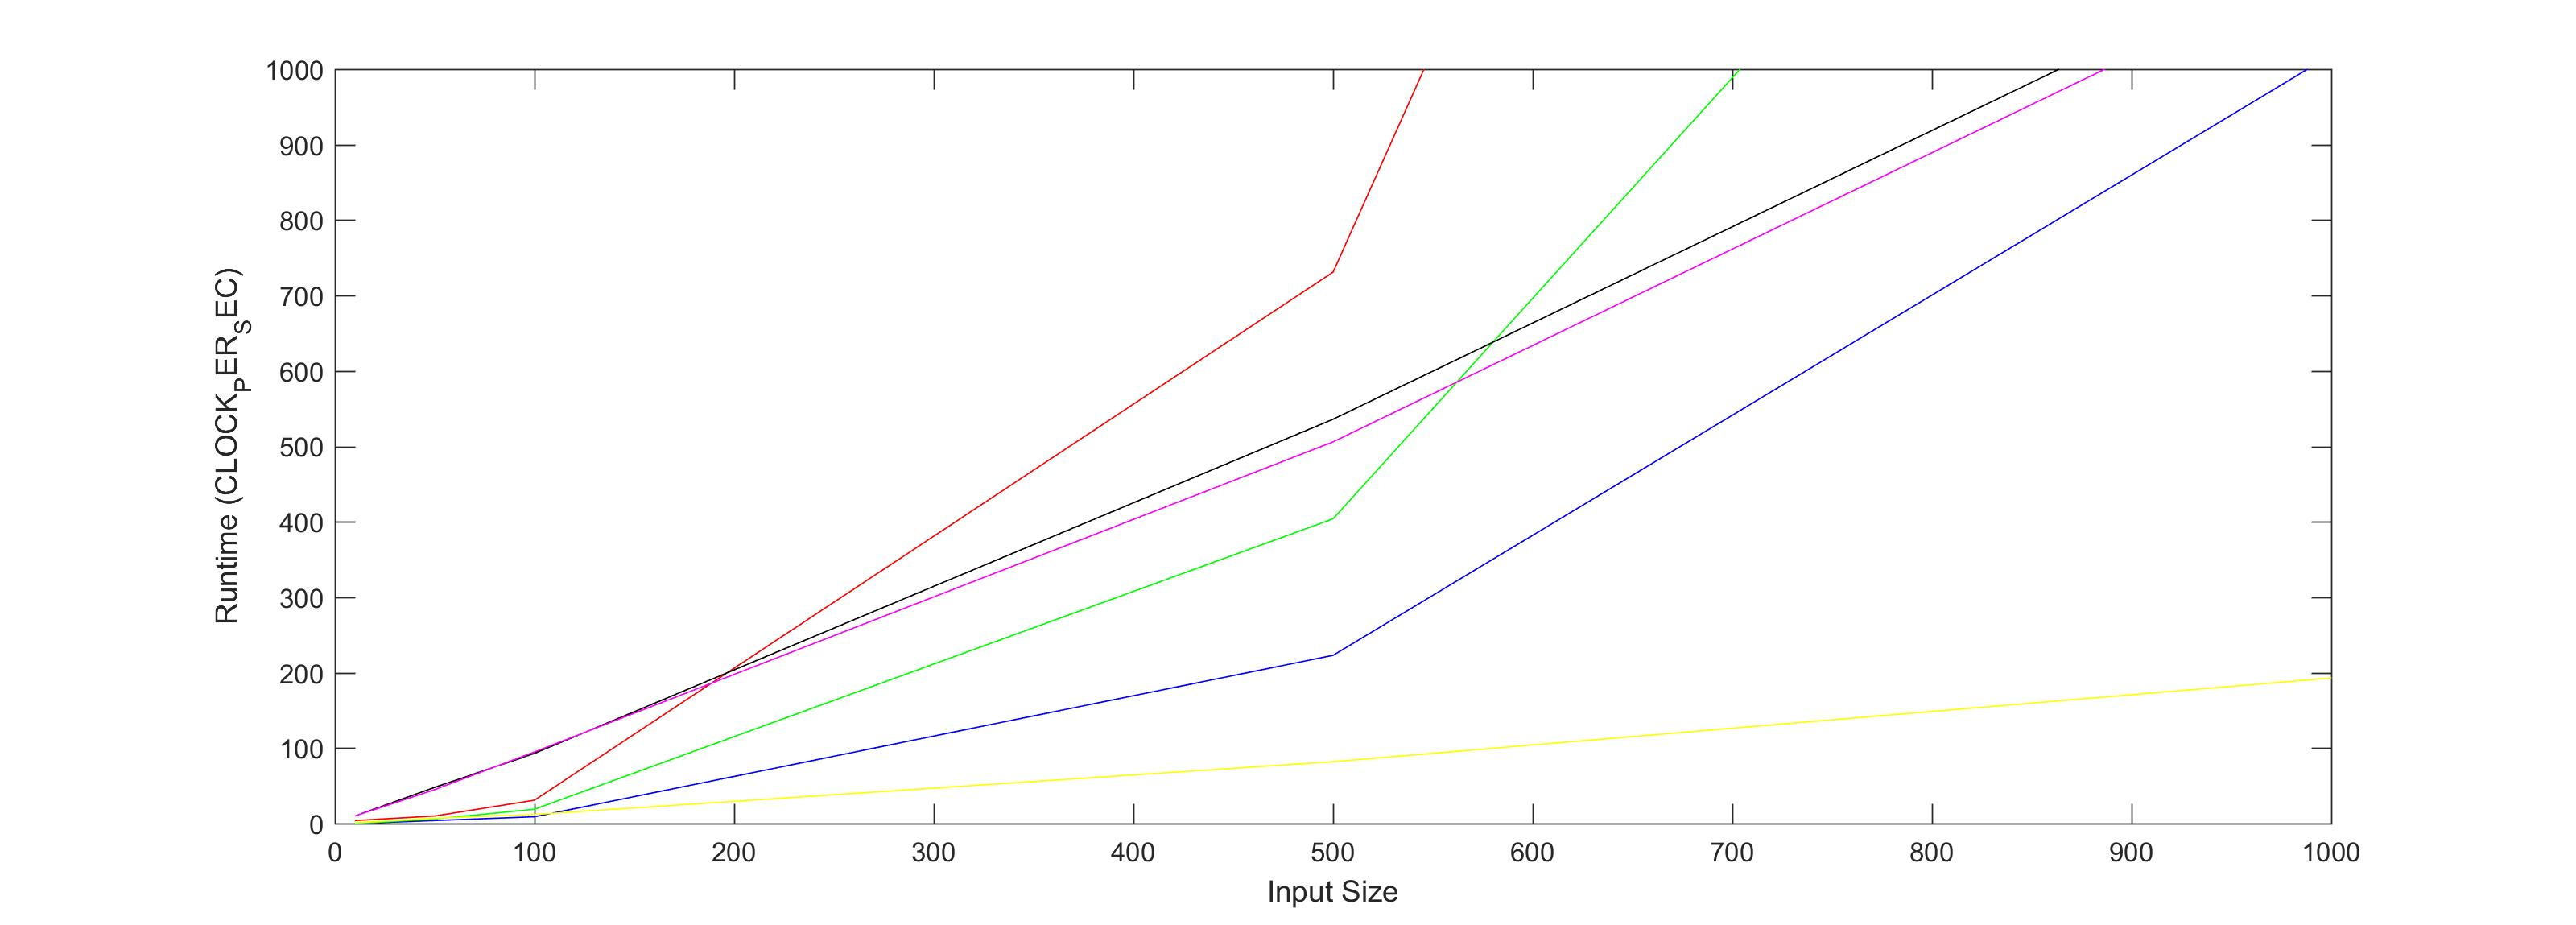
\includegraphics[width=\textwidth]{2.jpg}
\caption{Runtime of each algorithm versus the array size (small input size).}
\end{figure}
\begin{figure}[H]
\centering
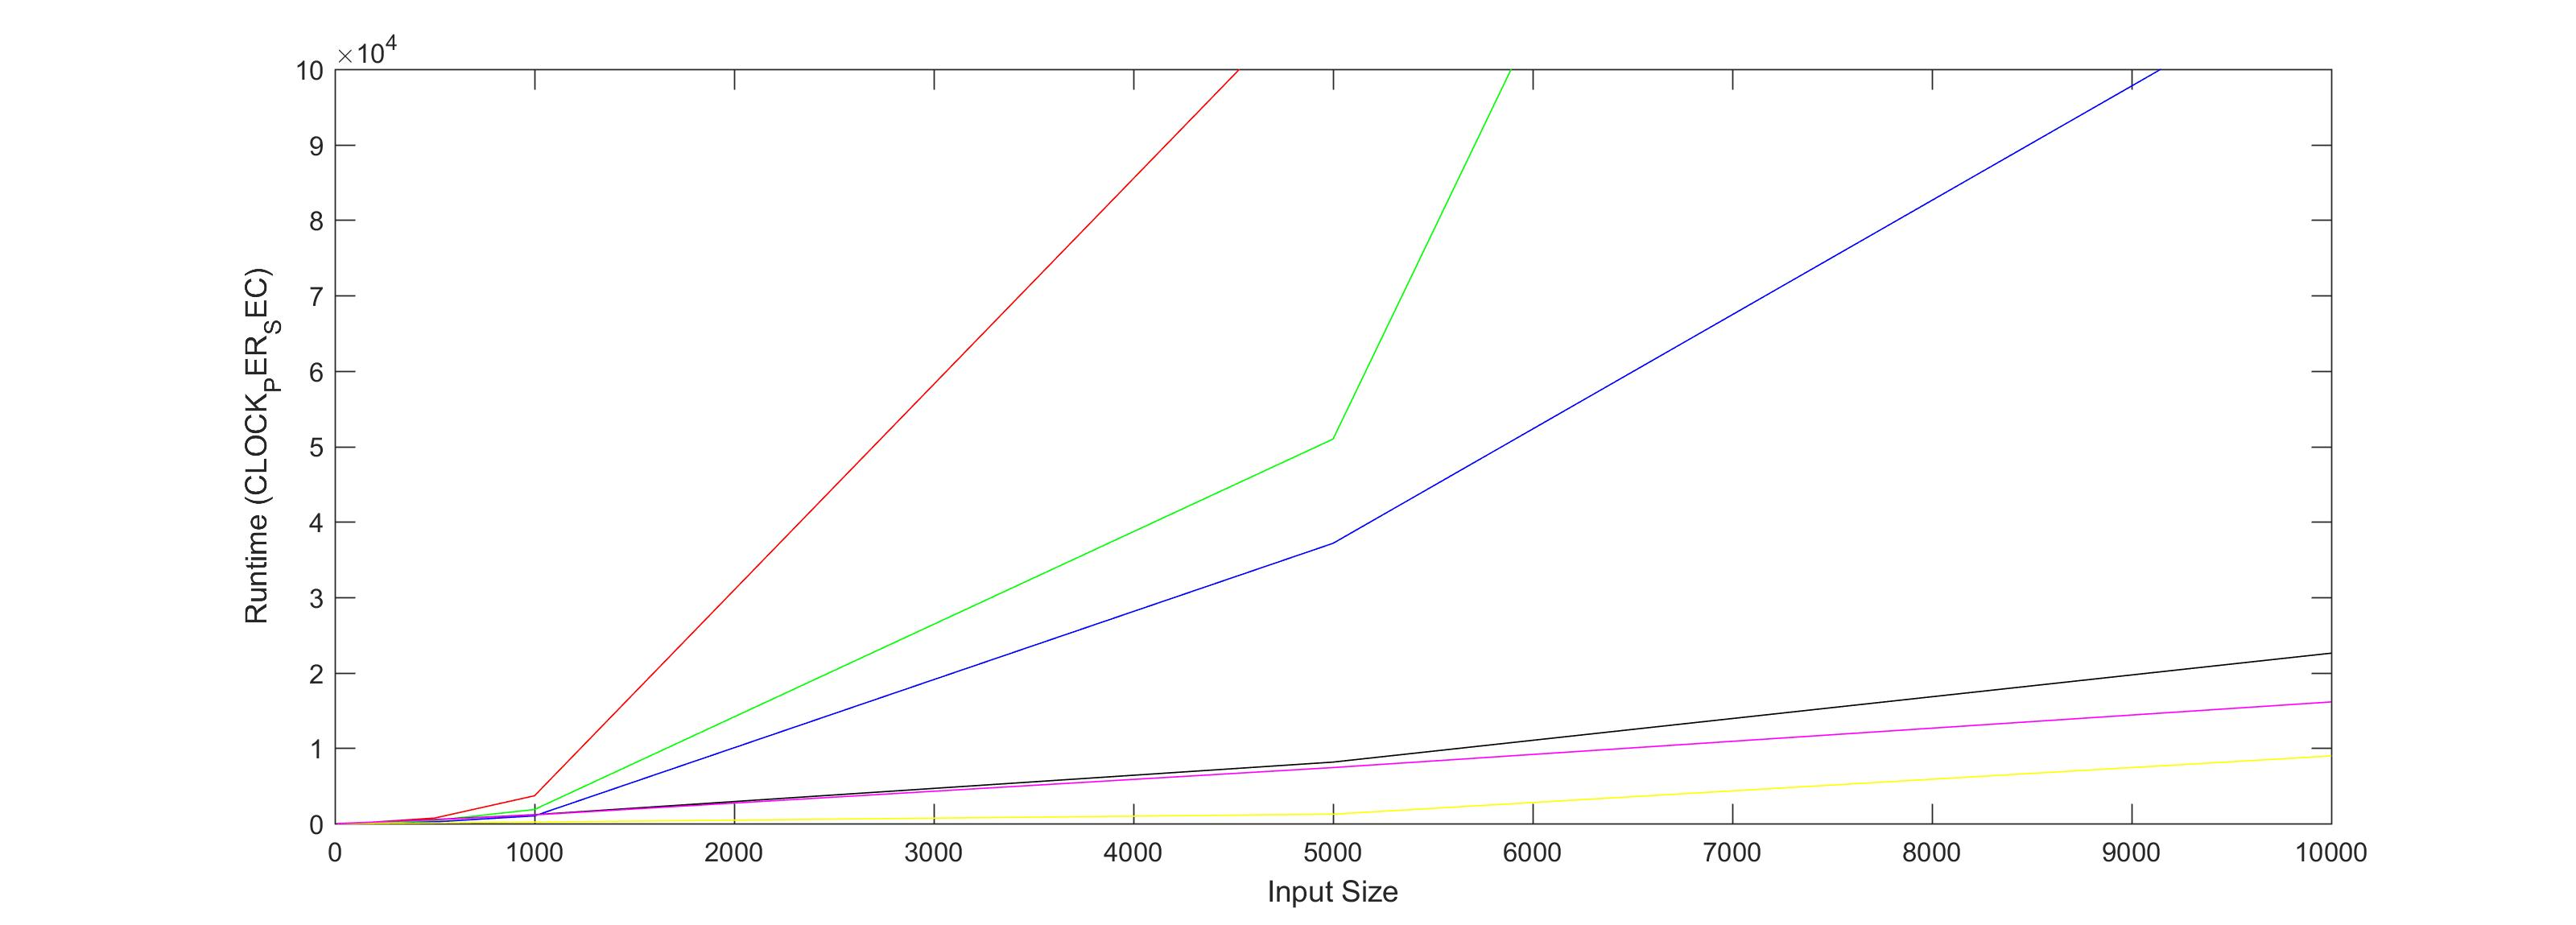
\includegraphics[width=\textwidth]{3.jpg}
\caption{Runtime of each algorithm versus the array size (middle input size).}
\end{figure}
In all three figures, red line represents the relationship between input size and runtime of bubble sort. Blue line represents the relationship between input size and runtime of insertion sort. Green line represents the relationship of selection sort. Yellow line represents the relationship of merge sort. Black line represents the relationship of quick sort with extra array while the purple one represents the relationship of quick sort with in-place partitioning.\\
\section{Discussion and Conclusion}
As we can see from three figures, merge sort and quick sort with extra array or in-place partitioning are much quicker than other three sorting algorithms, especially when the input size grows rapidly. We already know the time complexity from lecture. The average time complexity of bubble, selection and insertion sorting algorithms is $O(N^2)$ while the average time complexity of merge, quick sort with extra array and quick sort with in-place partitioning is only $O(N\log N)$. It shows the result of our test for the large input size is correct. \\
\\
From the result, we can also find that bubble sort is slowest. Compared with it, selection sort is much faster. And insertion sort is much faster than both two sorts. I think it shows that insertion sort is the quickest in all three simple sorts. For the large input size, merge sort and quick sort are quicker than all three simple sorts. The runtime is negligible. However, for small input size like 10, quick sort is slower than three simple sorts. With the growth of input size, the runtime of quick sort grows much slower than three simple sorts. As we can see from figure 2, the blue line is under black and purple lines for input size less than 10000, which satisfies the statement from the lecture that insertion sort is faster than quick sort for small arrays.\\
\\
Besides, I also find the runtime of quick sort with extra array is approximate to the runtime of quick sort with in-place partitioning. I think it can be concluded that the difference of two ways of quick sorts is how to find the correct place of pivot and the extra memory it needs. From figure 2 and figure 3, we can also find that the yellow line is always under black one and purple one, which represents that merge sort is faster than quick sort. I think it may be because of the worst case of quick sort. As we learned from lecture, the worst case time of merge sort is $O(N\log N)$ while the worst case time of quick sort is $O(N^2)$. We only test 50 times for each input size. It may be not many enough for the large input size.\\
\\
Due to the limitation of my computer, I cannot check the runtime of different sorting algorithms for some larger input sizes. But I think the tendency of lines in figure shows the result for larger input sizes. I think this check help me understand different sorting algorithms and time complexity better. It also makes me know the importance of time complexity. With computation of time complexity we can estimate the runtime of an algorithm before we run it. It is significant for some large input sizes and complex algorithms which may take long time.\\
\section{Appendix}
time.cpp\\
\#include $<$iostream$>$\\
\#include $<$fstream$>$\\
\#include $<$sstream$>$\\
\#include $<$string$>$\\
\#include $<$cstdlib$>$\\
\#include $<$climits$>$\\
\#include $<$ctime$>$\\
\#include $<$cassert$>$\\
\#include "sort.h"\\
\\
using namespace std;\\
\\
int main()\\
\{\\
    srand((unsigned)time(NULL));\\
    string name[6];\\
    name[0]="bubble   ";\\
    name[1]="insertion";\\
    name[2]="selection";\\
    name[3]="merge    ";\\
    name[4]="quick\_ex ";\\
    name[5]="quick\_in ";\\
    int n=10;\\
    clock\_t t[6];\\
    clock\_t tem;\\
    int s,r;\\
    int round=0;\\
    while (round$<$9)\\
    \{\\
    long int *a0,*a1,*a2,*a3,*a4,*a5;\\
    a0=new long int [n];\\
    a1=new long int [n];\\
    a2=new long int [n];\\
    a3=new long int [n];\\
    a4=new long int [n];\\
    a5=new long int [n];\\
    for (int i=0;i$<$6;i++) t[i]=0;\\
    s=0;\\
    r=0;\\
    while (r$<$50)\\
    \{\\
	  for (int i=0;i$<$n;i++) \{a0[i]=mrand48();a1[i]=a0[i];a2[i]=a0[i];a3[i]=a0[i];a4[i]=a0[i];a5[i]=a0[i];\}\\
	  while (s$<$6)\\
	  \{\\
	      tem=clock();\\
	      switch (s)\\
	      \{\\
		  case 0: bubble(\&a0[0],n);break;\\
		  case 1: insertion(\&a1[0],n);break;\\
		  case 2: selection(\&a2[0],n);break;\\
		  case 3: mergesort(\&a3[0],0,n-1);break;\\
		  case 4: quick\_extra(\&a4[0],0,n-1);break;\\
		  case 5: quick\_inplace(\&a5[0],0,n-1);break;\\
	      \}\\
	      tem=clock()-tem;\\
	      t[s]=(r*t[s]+tem)/(r+1);\\
              s++;\\
	  \}\\
	  r++;\\
    \}\\
    cout$<<$endl$<<$"Input size is "$<<$n$<<$endl;\\
    for (int i=0;i$<$6;i++) cout$<<$name[i]$<<$":\t"$<<$t[i]$<<$" CLOCK\_PER\_SEC"$<<$endl;\\
    delete [] a0;\\
    delete [] a1;\\
    delete [] a2;\\
    delete [] a3;\\
    delete [] a4;\\
    delete [] a5;\\
    if (round\%2==0) n=n*5;\\
    else n=n*2;\\
    round++;\\
    \}\\
\}\\
\\
\\sort.h\\
\#ifndef \_\_SORT\_H\_\_\\
\#define \_\_SORT\_H\_\_\\
\\
void bubble(long int *a, int len);\\
\\
void insertion(long int *a, int len);\\
\\
void selection(long int *a, int len);\\
\\
void mergesort(long int *a, int left, int right);\\
\\
void merge(long int *a, int left, int mid, int right);\\
\\
void quick\_extra(long int *a, int left, int right);\\
\\
void quick\_inplace(long int *a, int left, int right);\\
\\
int partition\_ex(long int *a, int left, int right);\\
\\
int partition\_in(long int *a, int left, int right);\\
\\
\#endif // \_\_SORT\_H\_\_\\
\\
\\
sort.cpp\\
\#include $<$iostream$>$\\
\#include $<$fstream$>$\\
\#include $<$sstream$>$\\
\#include $<$string$>$\\
\#include $<$cstdlib$>$\\
\#include $<$climits$>$\\
\#include $<$ctime$>$\\
\#include $<$cassert$>$\\
\#include "sort.h"\\
\\
using namespace std;\\
\\
void bubble(long int *a, int len)\\
\{\\
    long int tem;\\
    for (int i=len-2;i$>$=0;i--)\\
    \{\\
        for (int j=0;j$<$=i;j++)\\
        \{\\
            if (a[j]$>$a[j+1])\\
            \{\\
                tem=a[j];\\
                a[j]=a[j+1];\\
                a[j+1]=tem;\\
            \}\\
        \}\\
    \}\\
\}\\
\\
void insertion(long int *a, int len)\\
\{\\
    long int tem,j;\\
    for (int i=1;i$<$len;i++)\\
    \{\\
        tem=a[i];\\
        j=i-1;\\
        while ((j$>$-1)\&\&(tem$<$a[j]))\\
        \{\\
            a[j+1]=a[j];\\
            j--;\\
        \}\\
        a[j+1]=tem;\\
    \}\\
\}\\
\\
void selection(long int *a, int len)\\
\{\\
    long int tem,k;\\
    for (int i=0;i$<$len-1;i++)\\
    \{\\
        k=i;\\
        for (int j=i+1;j$<$len;j++)\\
        \{\\
            if (a[k]$>$a[j]) k=j;\\
        \}\\
        tem=a[i];\\
        a[i]=a[k];\\
        a[k]=tem;\\
    \}\\
\}\\
\\
void mergesort(long int *a, int left, int right)\\
\{\\
    if (left$>$=right) return;\\
    int mid=(left+right)/2;\\
    mergesort(a,left,mid);\\
    mergesort(a,mid+1,right);\\
    merge(a,left,mid,right);\\
\}\\
\\
void merge(long int *a, int left, int mid, int right)\\
\{\\
    int i,j,k;\\
    i=0;\\
    j=0;\\
    k=0;\\
    int sizeA, sizeB;\\
    sizeA=mid-left+1;\\
    sizeB=right-mid;\\
    long int tem[sizeA+sizeB];\\
    while ((i$<$sizeA)\&\&(j$<$sizeB))\\
    \{\\
        if (a[left+i]$<$=a[mid+1+j]) \{tem[k]=a[left+i];i++;\}\\
        else \{tem[k]=a[mid+1+j];j++;\}\\
        k++;\\
    \}\\
    if (i==sizeA)\\
    \{\\
        while (j$<$sizeB)\\
        \{\\
            tem[k]=a[mid+1+j];\\
            j++;\\
            k++;\\
        \}\\
    \}\\
    else\\
    \{\\
        while (i<sizeA)\\
        \{\\
            tem[k]=a[left+i];\\
            i++;\\
            k++;\\
        \}\\
    \}\\
    for (i=0;i$<$sizeA+sizeB;i++)\\
        a[left+i]=tem[i];\\
\}\\
\\
void quick\_extra(long int *a, int left, int right)\\
\{\\
    int pivotat;\\
    if (left$>$=right) return;\\
    pivotat=partition\_ex(a,left,right);\\
    quick\_extra(a,left,pivotat-1);\\
    quick\_extra(a,pivotat+1,right);\\
\}\\
\\
void quick\_inplace(long int *a, int left, int right)\\
\{\\
    int pivotat;\\
    if (left$>$=right) return;\\
    pivotat=partition\_in(a,left,right);\\
    quick\_inplace(a,left,pivotat-1);\\
    quick\_inplace(a,pivotat+1,right);\\
\}\\
\\
int partition\_ex(long int *a, int left, int right)\\
\{\\
    srand((unsigned)time(NULL));\\
    int p=rand()\%(right-left+1)+left;\\
    long int b[right-left+1];\\
    long int l,r,tem;\\
    tem=a[left];\\
    a[left]=a[p];\\
    a[p]=tem;\\
    l=0;r=right-left;\\
    int i=left+1;\\
    while (l$<$r)\\
    \{\\
        if (a[i]$<$a[left]) \{b[l]=a[i];l++;\}\\
        else \{b[r]=a[i];r--;\}\\
        i++;\\
    \}\\
    b[l]=a[left];\\
    for (i=left;i$<$=right;i++)\\
        a[i]=b[i-left];\\
    return l+left;\\
\}\\
\\
int partition\_in(long int *a, int left, int right)\\
\{\\
    srand((unsigned)time(NULL));\\
    int i=left+1, j=right;\\
    int p=rand()\%(right-left+1)+left;\\
    long int tem;\\
    tem=a[p];\\
    a[p]=a[left];\\
    a[left]=tem;\\
    if (i==j)\\
    \{\\
	if (a[left]$>$a[right])\\
	\{\\
	    tem=a[left];\\
	    a[left]=a[right];\\
	    a[right]=tem;\\
	\}\\
	else j--;\\
    \}\\
    else while (i$<$j)\\
    \{\\
        while ((i$<$right)\&\&(a[i]$<$a[left])) i++;\\
        while ((j$>$left)\&\&(a[j]$>$=a[left])) j--;\\
        if (i$<$j) \{tem=a[i];a[i]=a[j];a[j]=tem;\}\\
        else \{tem=a[j];a[j]=a[left];a[left]=tem;\}\\
    \}\\
    return j;\\
\}\\
\\
\end{document}
